\documentclass[12pt, twoside]{article}
\usepackage{jmlda}
\usepackage{NotationStyle}

\usepackage{pdfpages}
\usepackage{wasysym}
\usepackage{amsmath, amsfonts, amssymb}

\usepackage{graphicx}
\usepackage{longtable}
\usepackage{booktabs}

\usepackage{icomma}

\newcommand{\hdir}{.}

\newtheorem{hop}{Гипотеза}

\newtheorem{definition}{Определение}

\begin{document}

\title
    {Поиск границ радужки методом круговых проекций} % окончательное ли название?
\author
    {А.\,А.~Баженов, И.\,А.~Матвеев} % основной список авторов, выводимый в оглавление
\email
    {bazhenov.aa@phystech.edu; ivanmatveev@mail.ru}
%\thanks
%    {Работа выполнена при
%     %частичной
%     финансовой поддержке РФФИ, проекты \No\ \No 00-00-00000 и 00-00-00001.}
%\organization
%    {$^1$Организация, адрес; $^2$Организация, адрес}
\abstract
    {В работе решается задача нахождения границ радужки глаза по  изображению и примерной позиции зрачка. Для нахождения границ используются нейронные сети. Для понижения размерности используется метод круговых проекций яркости. Круговые проекции~--- интегралы градиента яркости изображения по концентрическим окружностям. Искомые границы соответствуют локальным максимумам зависимости круговой проекции яркости от радиуса. Зависимость непрерывная и имеет два ярко выраженных максимума и шумовую компоненту. Поэтому для анализа проекций используются методы, разработанные для анализа временных рядов. Для проверки качества работы алгоритма используется датасет ND-IRIS.
	
\bigskip
\noindent
\textbf{Ключевые слова}: \emph {круговые проекции, радужка, понижение размерности}

}

%данные поля заполняются редакцией журнала
%\doi{10.21469/22233792}
%\receivedRus{01.01.2017}
%\receivedEng{January 01, 2017}

\maketitle
\linenumbers

\section{Введение}
В работе рассматривается один из этапов идентификации человека по радужке, описанной в [1, 2]. Распознавание требует предварительную сегментацию изображения глаза.

В [3] описан алгоритм сегментации глаза. Упрощенная схема работы алгоритма:
\begin{enumerate}
	\item Нахождение центра зрачка.
	 Расстояние между найденным и истинным центрами не превышает половину радиуса зрачка.
	\item Нахождение приблизительных границ зрачка и радужки.
	На этом этапе границы представляются окружностями, центры которых совпадают с найденным на предыдущем этапе центром зрачка. Отличие найденного и истинного радиусов не превышает $10\%$.
	
	\item Уточнение найденных ранее центра и границ.
\end{enumerate}
Для реализации второго этапа в [3,4] предлагается использовать метод круговых проекций яркости с последующим эвристическим выбором наиболее подходящих радиусов.
\begin{definition}\label{def:proj}
\emph{Круговой проекцией яркости} называется интеграл градиента яркости по дуге окружности.
\end{definition}
В [4] высказывается предположение, что радиус границы является точкой локального максимума круговой проекции яркости. Однако, неоднородности изображения создают большое число точек локального максимума. В [4] проблема решена эвристическим выбором из локальных максимумов. Такое решение показывает неусточивость к шумовым факторам, например, к теням от ресниц.

Данная работа рассматривает возможные замены эвристическому выбору. Зависимость круговой проекции от радиуса окружности похожа на временной ряд. Исходя из этого, используются методы, предложенные в [5] для обработки временных рядов: реккурентные и сверточные нейронные сети. Модели сравниваются с полносвязной нейронной сетью. В результате многократного повторения процедуры обучения моделей, выявлено, что рекуррентная и сверточная сеть более подвержены случайностям ,чем полносвязная модель, но показывают лучшую точность.

\section{Постановка задачи}
\subsection{Система нахождения границ радужки}

Рассматриваются данные в виде растрового изображения глаза $M$. Изображение представляет из себя зрачок~--- круг с центром в точке $\begin{bmatrix}P_x & P_y\end{bmatrix}\T$ и радиусом $P_\text{R}$, окруженный радужкой~--- кругом с центром в точке $\begin{bmatrix}I_x & I_y\end{bmatrix}\T$ и радиусом $I_\text{R}$, часть которого может отсутствовать на изображении. В дальнейшем будем называть $P_\text{R}$ \textit{радиусом границы зрачка}, а $I_\text{R}$~--- \textit{радиусом границы радужки}. Помимо зрачка и радужки, на изображении присутсвуют посторонние элементы.

\begin{definition}
\emph{Система нахождения границ радужки}~--- это отображение
\[f\!: \quad M \mapsto \begin{bmatrix}\widehat{P}_\text{R} &  \widehat{I}_\text{R}\end{bmatrix}\T.\]
\end{definition}
В работе рассматривается задача приблизительного нахождения границ, поэтому малые отклонения результата работы системы от истинного значения не должны штрафоваться, а большие отклонения должны штрафоваться сильно. Рассматривается кусочно-линейная функция
\[
h_{\alpha, \beta}(t) = \begin{cases}0, &t < \alpha, \\ t - \alpha, &\alpha \leqslant t < \beta, \\ (\beta - \alpha) + 5\cdot (t - \beta), & t > \beta.\end{cases}
\]
Используемая в работе функция потерь~--- результат композиции функции $h_{\alpha, \beta}$ и функции относительного отклонения
\[
L_{\alpha, \beta} (x, y) = h_{\alpha, \beta}\left(\frac{|x-y|}{y}\right).
\]
По экспертным соображениям, были выбраны значения $\alpha = 0.1$ и $\beta = 0.2$. Рассматривается задача оптимизации
\begin{equation}\label{mainproblem}
\sum_{i=1}^n \left[ L_{\alpha, \beta} \left(\widehat{P}_\text{R}(i), P_\text{R}(i)\right) + L_{\alpha, \beta} \left(\widehat{I}_\text{R}(i), I_\text{R}(i)\right) \right]\to \min_{f\in \mathcal{F}},
\end{equation}
вид множества допустимых моделей $\mathcal{F}$ описывается в разделе 2.3.

\subsection{Метод круговых проекций}
Обозначим $\vec{x} = (x, y)$~--- точку на изображении, $b(\vec{x})$~--- яркость изображения в этой точке, $\vec{g}(\vec{x}) = \nabla b(\vec{x})$~--- градиент яркости. Согласно предположению, указанному в статье [4], точки, лежащие на границе радужки либо зрачка, должны удовлетворять условию, описываемому индикаторной функцией:
\[
v_U(\vec{x}) = \begin{cases}1, & \| \vec{g} \| > T_1 \text{ и } \frac{(\vec{x}, \vec{g})}{\| x \| \cdot \| g \|} > T_2 \text{ и } \vec{x} \in U, \\ 0, & \text{ иначе.}\end{cases}
\]
Выбор пороговых значений $T_1$ и $T_2$ описан в [4]. Множество $U$~--- квадрант, то есть одно из множеств точек плоскости:
\[
U = \begin{cases}L\!: & |x| > |y| \text{ и } x < 0, \\ R\!: & |x| > |y| \text{ и } x > 0, \\ B\!: & |x| \leqslant |y| \text{ и } y < 0, \\ T\!: & |x| \leqslant |y| \text{ и } y > 0.\end{cases}
\]

При условии отсутствия неоднородностей на изображении глаза в граничных точках будет выполнено $v_U(\vec{x})=1$, в остальных будет выполнено $v_U(\vec{x})=0$. При применении же к реальным изображениям возможны двусторонние ошибки: $v_U(\vec{x})=1$ для неграничной точки, $v_U(\vec{x})=0$ для граничной точки. В первом приближении считается, что неоднородности не имеют структуры, значит события 
\[
A_x = \{\text{при классификации точки }x\text{ произошла ошибка}\}
\]
независимы. Тогда при усреднении индикаторов $v_U(\vec{x})$ по контуру предполагаемой границы вероятность ошибки классификации уменьшается. Такое усреднение выражается через дискретный случай определения~\ref{def:proj}:
\begin{definition}\label{def:proj_sum}
\emph{Круговая проекция яркости}~--- нормированная сумма индикаторных величин
\[
\Pi_U(r) = \frac{1}{2\pi r} \sum_{r-0.5 < \|x\|<r+0.5} v_U(x).
\] 
\end{definition}

\subsection{Ограничение на множество моделей}

Рассмотрим задачу нахождения радиусов границ радужки и зрачка при известном приблизительном положении центра зрачка. Обозначим $\Pi_U$~--- вектор значений круговых проекций яркости:
\[
\Pi_U = \begin{bmatrix}\Pi_U(1) & \ldots & \Pi_U(r_{\max})\end{bmatrix}\T.
\]
Обработку посчитанных значений проводится при помощи нейронной сети, то есть множество допустимых моделей имеет вид:
\[
\mathcal{F} = \{f = \sigma_k\large\left(\bW_k\T \sigma_{k-1}\large\left(\ldots \sigma_1\left(\bW_1\T \Pi_U\right)\ldots\large\right)\large\right)\}.
\] 

При фиксированной архитектуре нейронной сети, то есть при фиксированных $k$ и функциях активации $\sigma_1, \ldots, \sigma_k$ решается задача оптимизации среднеквадратичного отклонения
\begin{equation}\label{secondproblem}
\frac{1}{n}\sum_{i=1}^n \left[\left(\widehat{P}_\text{R}(i) - P_\text{R}(i)\right)^2 + \left(\widehat{I}_\text{R}(i) - I_\text{R}(i)\right)^2\right] \to \min_{W_1, \ldots, W_k}.
\end{equation}

\section{Нахождение радиусов границ}

\begin{figure}[!htbp]
	\centering
	\includegraphics[scale=0.4]{img/projs.pdf}
	\caption{Круговые проекции яркости для одного из изображений}
	\label{fig:projs}
\end{figure}

Пусть считается известной зависимость значения круговой проекции яркости от радиуса $\Pi_U(r)$. Рассмотрим некоторые значения радиусов $r_1$ и $r_2$. Исходя из определения~\ref{def:proj_sum} делается предположение:
\begin{hop}
Если выполнено неравенство $\Pi_U(r_1) > \Pi_U(r_2)$, то вероятность наличия круговой границы радиуса $r_1$ больше, чем вероятность наличия границы радиуса $r_2$.
\end{hop}

На рис.~\ref{fig:projs} представлена зависимость круговой проекции яркости от радиуса окружности для изображения из выборки ND-IRIS. Реальные значения радиусов не совпадают с точками максимумов, поэтому гипотеза 1 не верна. Однако, пики зависимости не покрывают значения радиусов границ. Отсюда вытекает гипотеза 2.

\begin{hop}
Пусть $r^*$~--- радиус круговой границы. Тогда существует такая случайная величина $\xi$ , что
\[
 r^* = \arg \text{loc}\max\limits_{r}\Pi_U(r) + \xi, \quad \mathsf{E}\xi=0.
\]
\end{hop}

При работе в предположении верности гипотезы 2, задача сводится к поиску двух локальных максимумов зависимости. Окрестности максимумов также содержат информацию, обработка которой позволяет уточнить значения радиусов. Обработка круговых проекций яркости схожа с задачей выделения аномалий из непрерывной зависимости, поэтому в работе применяются нейронные сети, предложенные в [5] для обработки врменных рядов: сверточные и рекуррентные нейронные сети.

\subsection{Сверточная нейронная сеть}

\begin{figure}[!htbp]
\begin{center}
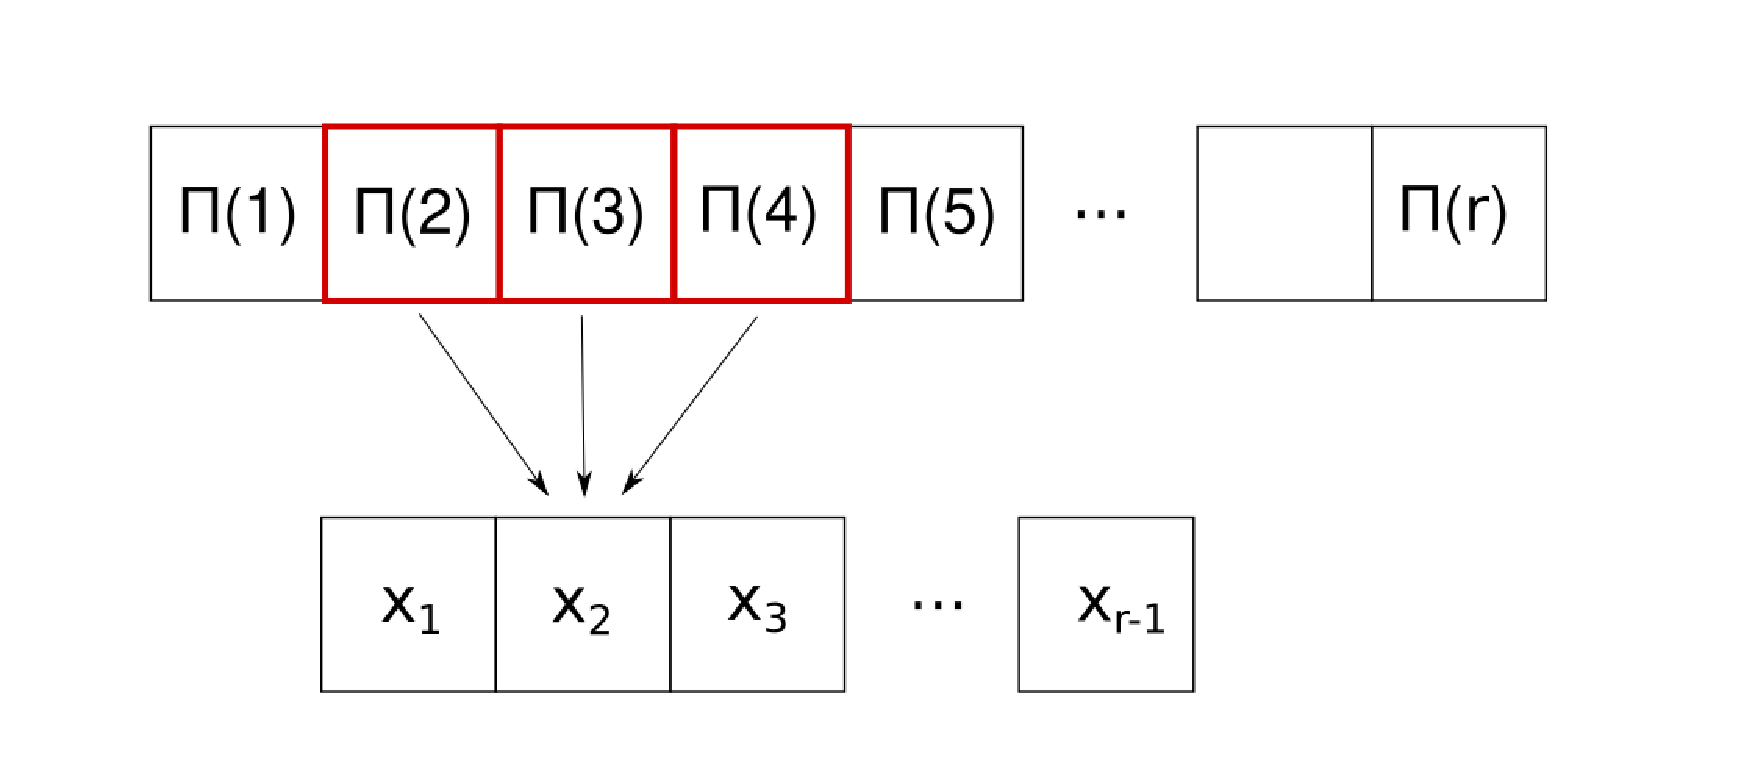
\includegraphics[scale=0.4]{fig/conv.pdf}
\end{center}
\caption{Схема обработки данных в сверточном слое}
\label{fig:conv}
\end{figure}
Круговые проекции яркости обрабатываются путем многократного применения линейных фильтров с обучаемыми коэффициентами, называемых \emph{сверточными слоями}. Схема работы сверточного слоя показана на рис.~\ref{fig:conv}. Линейный фильтр позволяет выявлять соотношения между соседними элементами вектора проекций, в частности выделять экстремумы зависимости $\Pi_U(r)$. При этом число обучаемых параметров сверточного слоя не зависит от размера входных данных, что уменьшает число обучаемых параметров в сравнении с полносвязным слоем. Полученные многократным применением сверток данные обрабатываются при помощи полносвязного слоя, число параметров в котором меньше, чем при применении полносвязного слоя к изначальным данным.

\subsection{Рекуррентная нейронная сеть}

Круговые проекции обрабатываются последовательно. При применении к входным данным преобразований, генерируются выходные данные и \emph{скрытое состояние сети} $H \in \mathbb{R}^d$. Скрытое состояние используется при обработке следующих элементов последовательности $\Pi_U$, что позволяет выделять экстремумы и обрабатывать их окрестности. Для последующей обработки используются как получившаяся последовательность скрытых состояний, так и новая последовательность данных.

\begin{figure}[!htbp]
\begin{center}
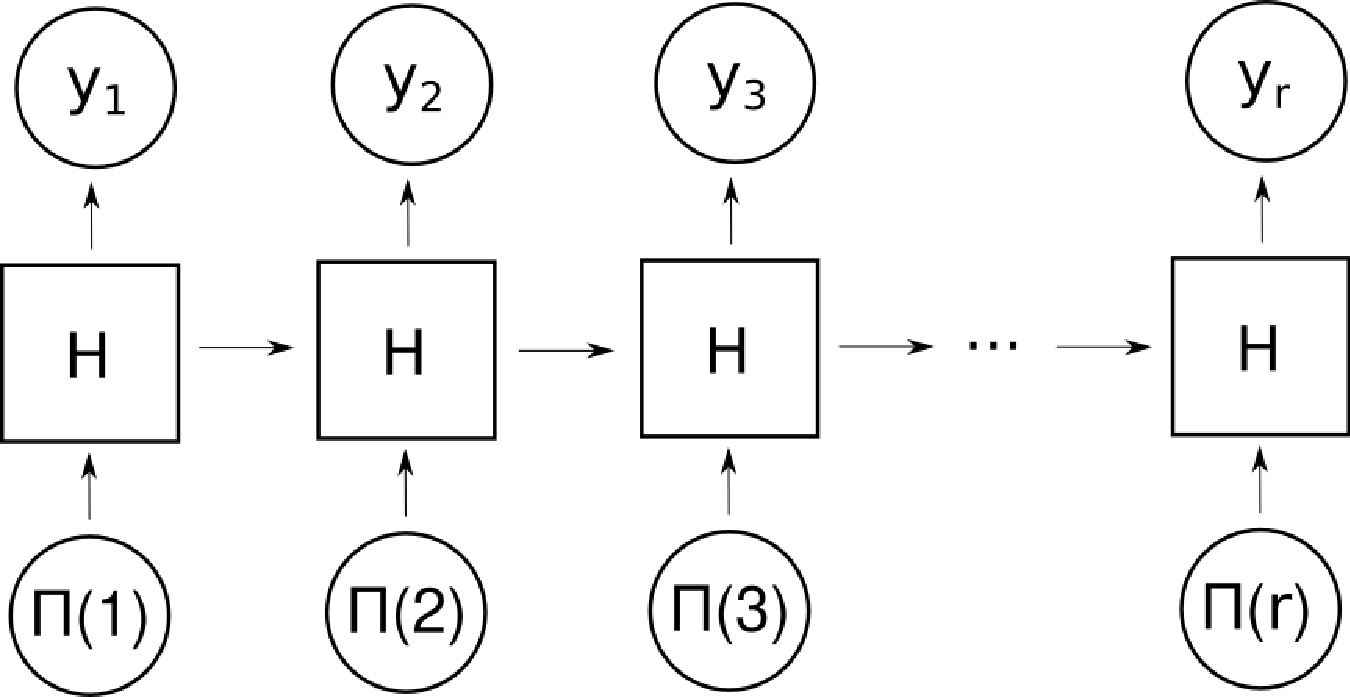
\includegraphics[scale=0.4]{fig/rnn.pdf}
\end{center}
\caption{Схема обработки данных в рекуррентной сети}
\label{fig:rnn}
\end{figure}

\section{Вычислительный эксперимент}

Проведение эксперимента заключается в оптимизации модели нейронной сети и последующем ее тестировании. Выборка изображений разделяется на три части: обучающую, валидационную и тестовую, размер которых относится как 4:1:1. Для всех изображений считаются круговые проекции яркости, считающиеся в дальнейшем исходными данными. Для каждой из архитектур, представленных в предыдущем пункте, а также для полносвязной модели решается задача оптимизации~\eqref{secondproblem}. Затем полученные модели сравниваются по значению функционала~\eqref{mainproblem}.

\textbf{Цель эксперимента}

Целью эксперимента является выявление наилучшей архитектуры по следующим параметрам:
\begin{enumerate}
	\item Качество решения задачи~\eqref{mainproblem};
	\item Устойчивость к малым изменениям исходных данных;
	\item Скорость работы алгоритма. Алгоритм должен позволять обрабытывать видеопоток с частотой кадров не менее 30 кадров в секунду.
\end{enumerate}

\textbf{Ход эксперимента}

\begin{figure}[!htbp]
	\centering
	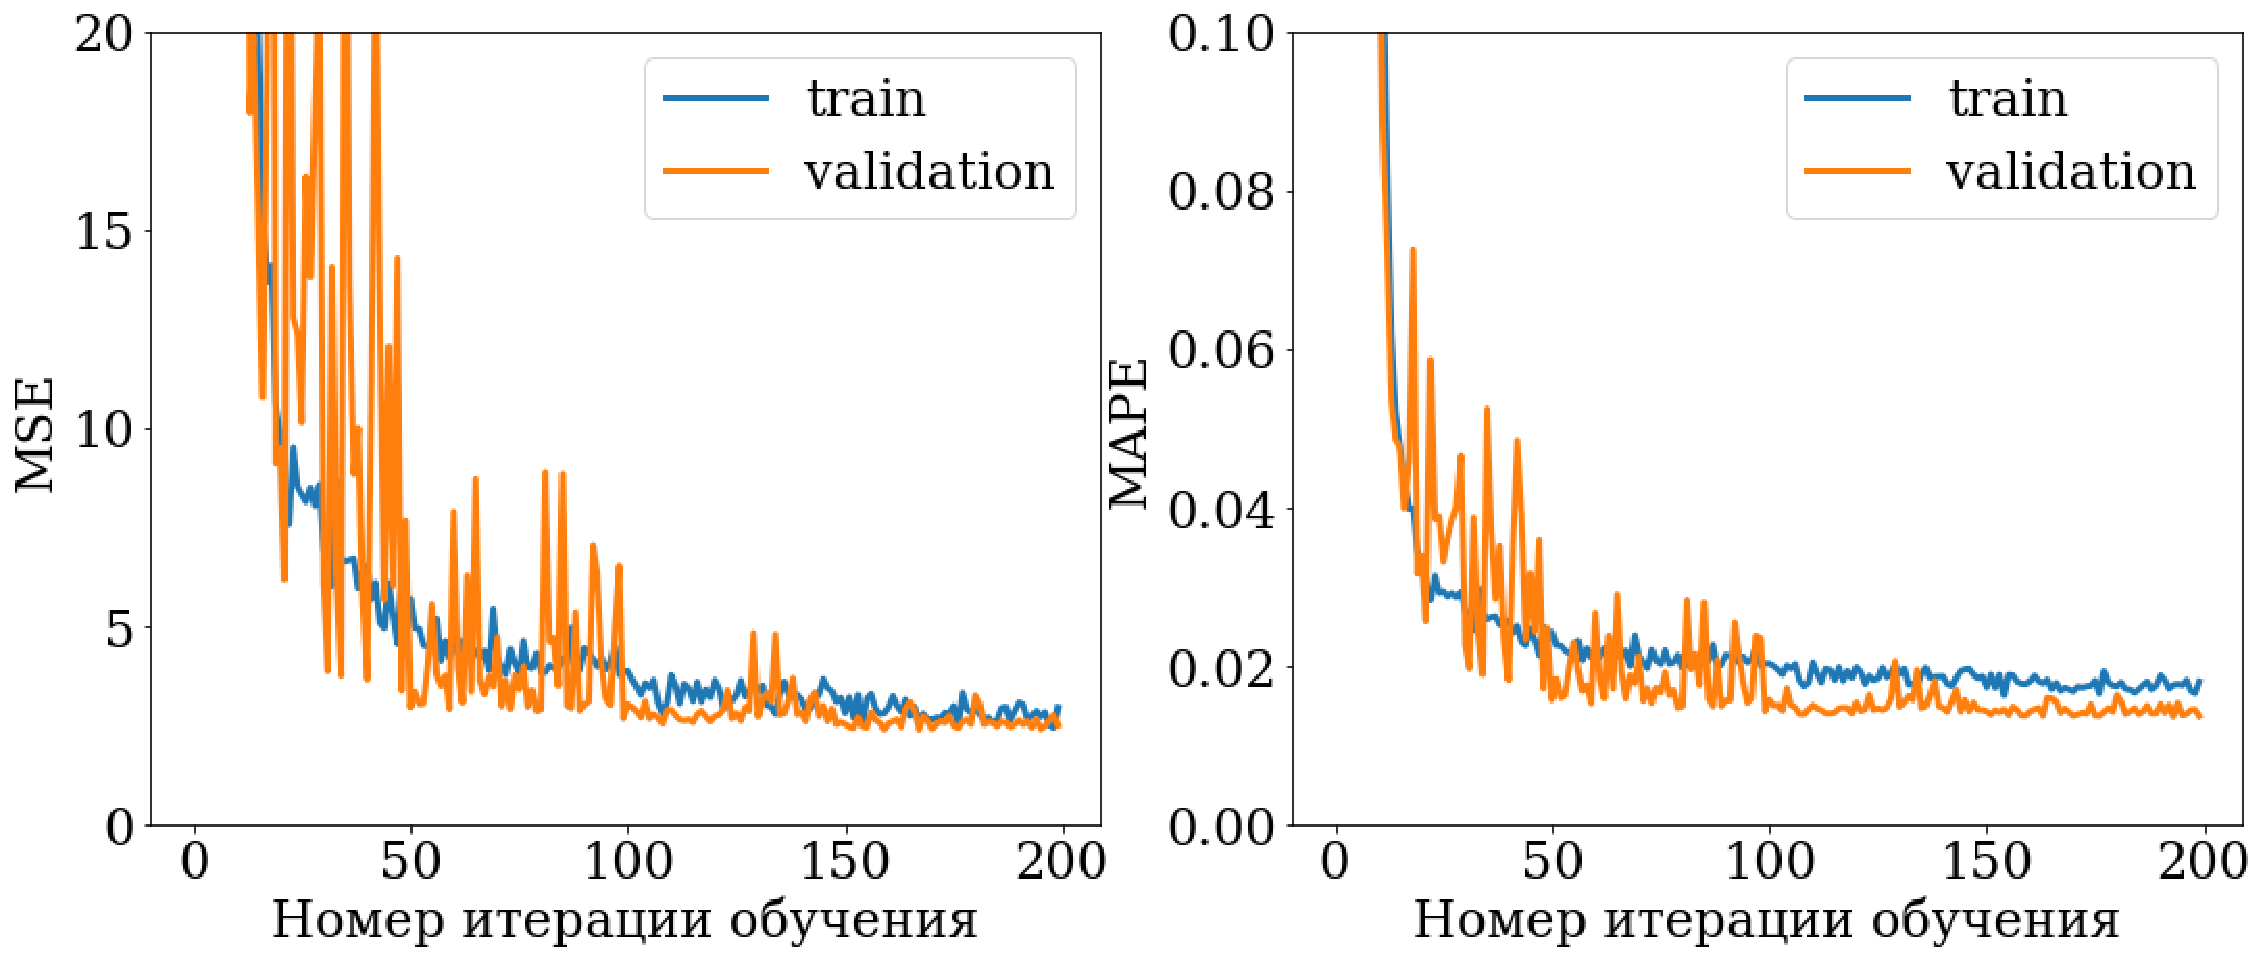
\includegraphics[scale=0.4]{img/single_experiment.pdf}
	\caption{Кривые обучения для сверточной модели}
	\label{fig:singleexp}
\end{figure}
Применялся алгоритм оптимизации Adam [6]. Параметры алгоритма подбирались так, чтобы значения функционалов MSE и MAPE показывали уменьшение на обучающей и валидационной выборках. Значение параметра learning rate уменьшалось каждые несколько итераций обучения для достижения лучшего качества моделей. Метрики для единичного запуска эксперимента для одной из сверточных моделей показаны на графике~\ref{fig:singleexp}. Графики для всех моделей находятся в репозитории проекта.


\textbf{Анализ ошибки}

\begin{figure}[!htbp]
	\centering
	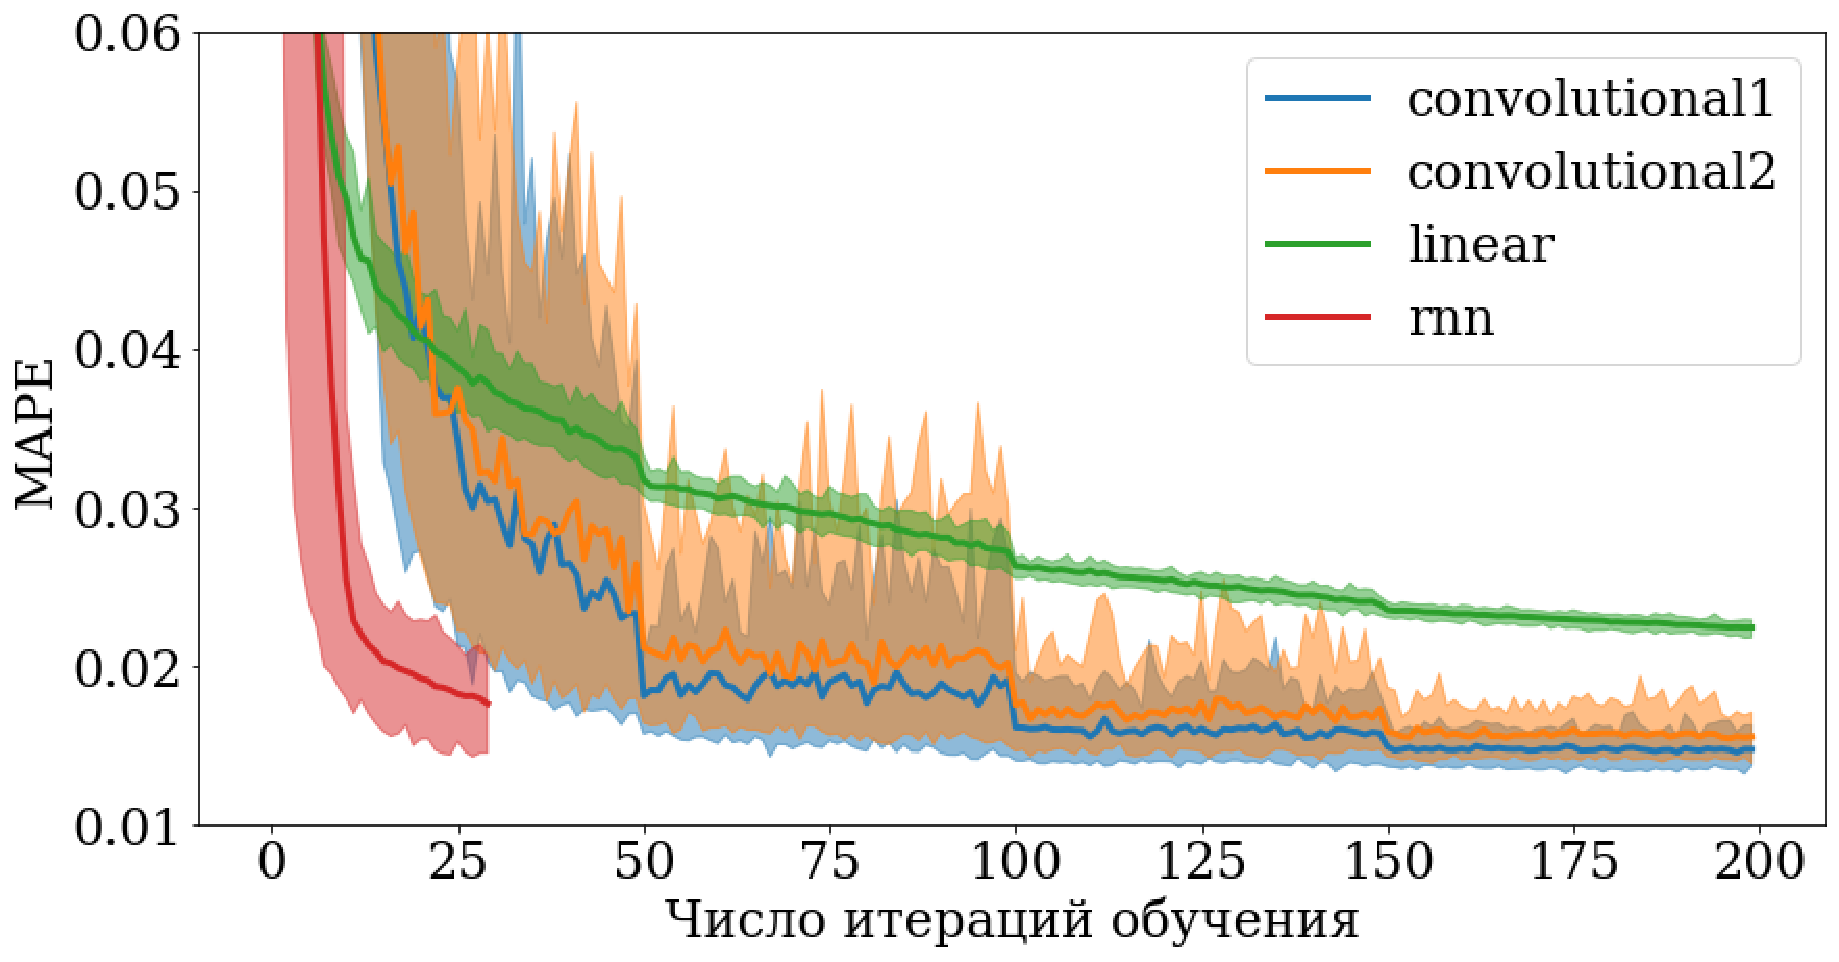
\includegraphics[scale=0.4]{img/multerror.pdf}
	\caption{Доверительный интервал ошибки на валидационной выборке}
	\label{fig:multerr}
\end{figure}
Было проведено 50 независимых запусков эксперимента. Полученные в результате доверительные интервалы ошибки отражены на графике~\ref{fig:multerr}.

Для каждого запуска эксперимента было посчитано итоговое качество на тестовой выборке. Результаты отображены в таблице~\ref{table:error}. По результатам эксперимента, реккурентная и сверточная модели показывают большую точность, чем полносвязная модель.

\begin{table}
\caption{Ошибка на тестовой выборке}
\label{table:error}
\begin{tabular}{c c c c}
\hline
Архитектура & Число \mbox{параметров} & Средняя ошибка, \% & Доверительный интервал\tabularnewline
\hline
Полносвязная & $166402$ & $2,21$ & $2,15$-$2,24$\tabularnewline
Сверточная & $56831$\ & $1,39$ & $1,32$-$1,47$\tabularnewline
Сверточная & $17655$ & $1,48$ & $1,39$-$1,58$\tabularnewline
Реккурентная & $14962$ & $1,77$ & $1,45$-$2,05$\tabularnewline
\hline
\end{tabular}
\end{table}


\section{Заключение}
Для решения задачи нахождения границ радужки используются метод круговых проекций и нейронные сети. В результате было выявлено, что нейронные сети, созданные для обработки временных рядов, показывают точность, достаточную для первого приближения, то есть превосходящую $10\%$. Применение методов, разработанных для анализа временных рядов, позволило получить большую точность, чем применение полносвязной модели, что подтверждает схожесть круговых проекций яркости и других

%%%% если имеется doi цитируемого источника, необходимо его указать, см. пример в \bibitem{article}
%%%% DOI публикации, зарегистрированной в системе Crossref, можно получить по адресу http://www.crossref.org/guestquery/
\begin{thebibliography}{99}


 \bibitem{article}
    \BibAuthor{A.~Nithya, C.~Lakshmi}
   Iris Recognition Techniques: A Literature Survey~//
    \BibJournal{International Journal of Applied Engineering Research}, 2015

 \bibitem{article}
    \BibAuthor{K.~Bowyer, K.~Hollingsworth, and P.~Flynn}
   Image Understanding for Iris Biometrics: A Survey~//
    \BibJournal{Computer Vision and Image Understanding}, 2008. Vol.~110. \No\,2. pp.~281--307
	
 \bibitem{article} 
    \BibAuthor{K.\,A.~Gankin, A.\,N.~Gneushev, and I.\,A.~Matveev}
   Iris image segmentation based on approximate methods
with subsequent refinements~//
    \BibJournal{Journal of Computer and Systems Sciences International}, 2014. Vol.~53. \No\,2. pp.~224--238.
	\BibDoi{10.1134/S1064230714020099}.
	
  \bibitem{article}
    \BibAuthor{I.\,A.~Matveev}
   Detection of iris in image by interrelated maxima of brightness gradient projections~//
    \BibJournal{Appl. Comput. Math.}, 2010. Vol.~9. \No\,2. pp.~252--257.
    
    \bibitem{article}
    \BibAuthor{B.~Lim, S.~Zohren}
    Time-series forecasting with deep learning: a survey~//
	\BibJournal{Philosophical Transactions of the Royal Society}, A 379: 20200209.
	\BibDoi{10.1098/rsta.2020.0209}
	
	\bibitem{article}
	\BibAuthor{D.\,P.~Kingma, J.\,L.~Ba}
	Adam: A Method for Stohastic Optimization~//
	\BibJournal{ICLR 2015}
	
	\bibitem{webResource}
	Исходный код проекта.
	URL: \BibUrl{https://github.com/Intelligent-Systems-Phystech/2021-Project88/}
 
 	
\end{thebibliography}

%%%% если имеется doi цитируемого источника, необходимо его указать, см. пример в \bibitem{article}
%%%% DOI публикации, зарегистрированной в системе Crossref, можно получить по адресу http://www.crossref.org/guestquery/.

\end{document}
